\subsection{Isosurface extraction}\label{sec:isocontour}

\begin{figure*}[h]
\centering
\subcaptionbox{\em pressure, isovalue=0.2}
{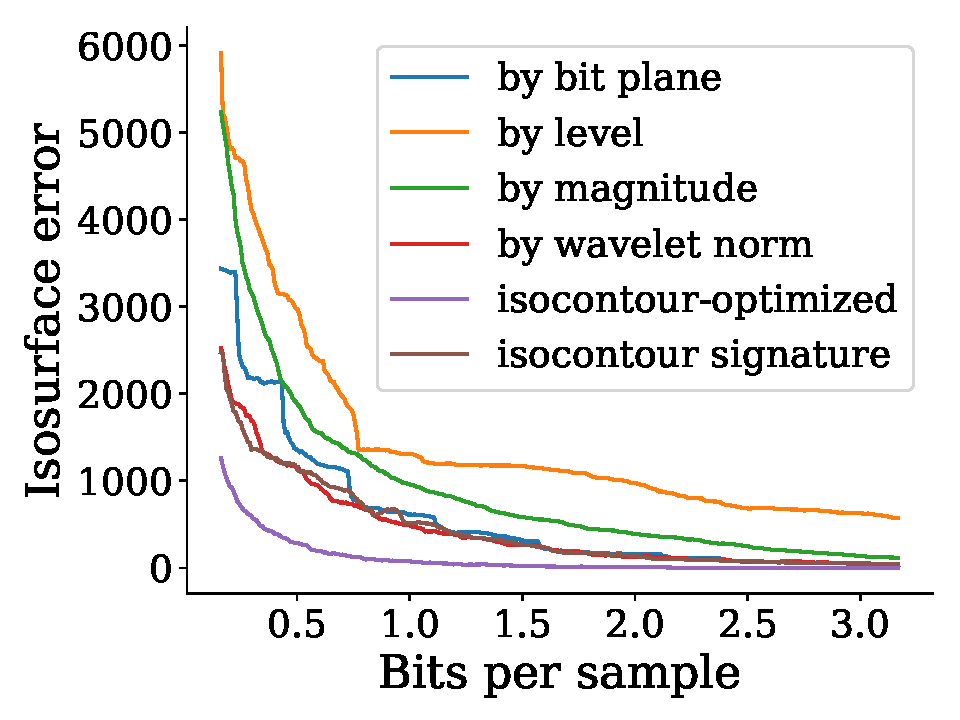
\includegraphics[width=0.24\linewidth]{isocontour/isocontour-optimized-pressure}}
\subcaptionbox{\em turbulence, isovalue=5}
{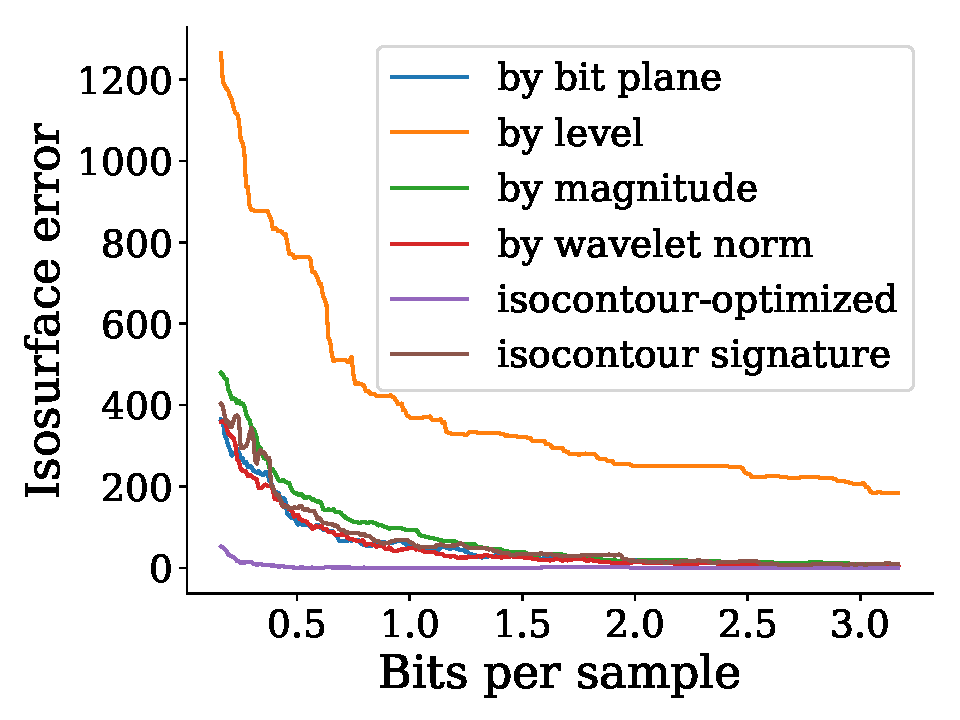
\includegraphics[width=0.24\linewidth]{isocontour/isocontour-optimized-turbulence}}
\subcaptionbox{\em plasma, isovalue=2}
{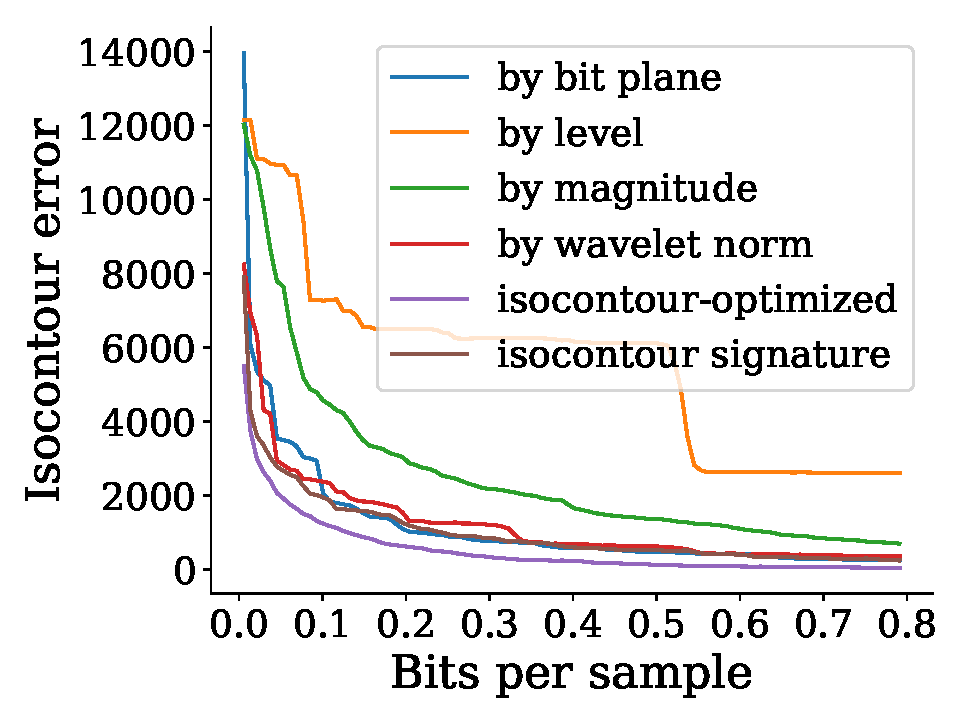
\includegraphics[width=0.24\linewidth]{isocontour/isocontour-optimized-plasma}}
\subcaptionbox{\em diffusivity, isovalue=-0.05}
{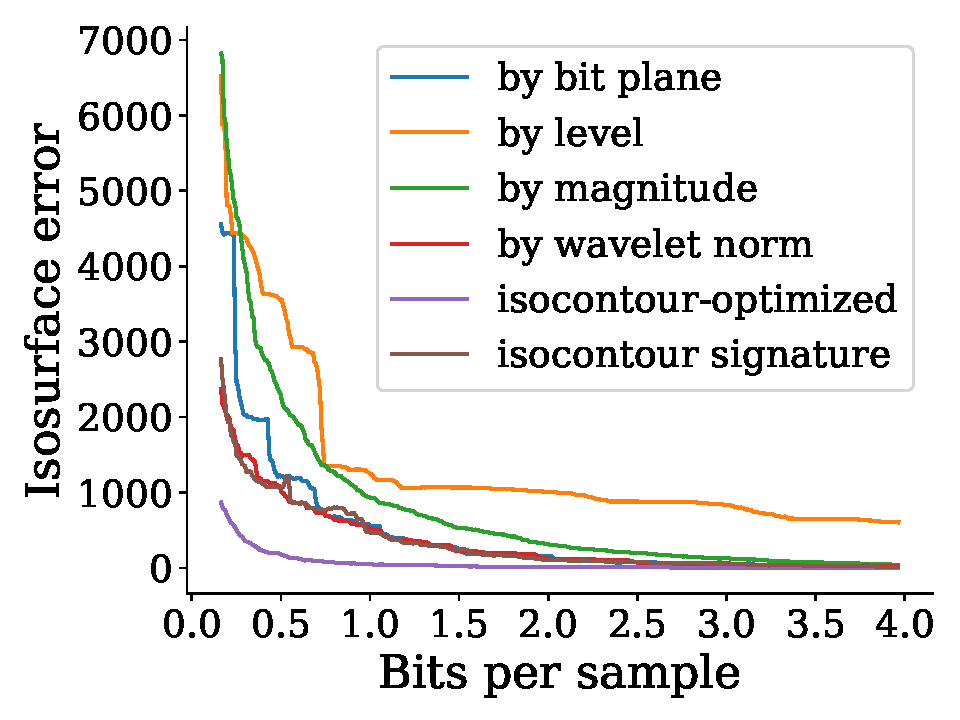
\includegraphics[width=0.24\linewidth]{isocontour/isocontour-optimized-diffusivity}}
\caption{Comparison of isosurface errors among streams. Plots are truncated to highlight differences
without hiding important trends. In all cases, \slvl and \smag perform significantly worse than the
rest. For \emph{pressure} and \emph{diffusivity}, in terms of error, $\sisg \approx \swav < \sbit$.
For \emph{plasma}, there are crossovers between \sbit and \swav. Finally, for \emph{turbulence},
$\sbit < \swav \approx \ssig$ in isosurface error.} \label{fig:isocontour-plots}
\vspace{1em}

\centering
\subcaptionbox{\emph{by level} ($s_{lvl}$)}
{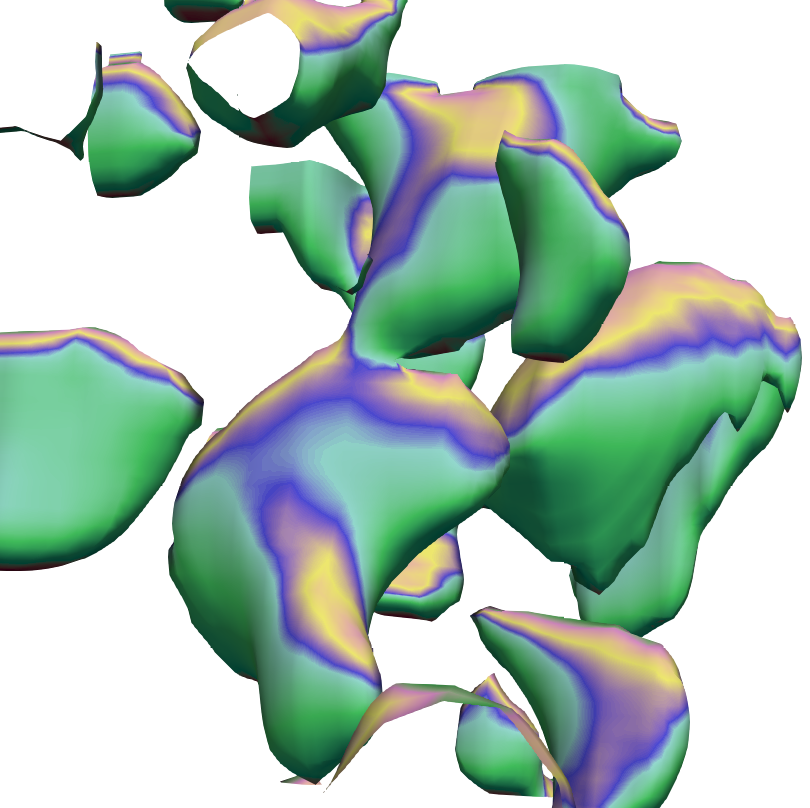
\includegraphics[width=0.16\linewidth]{isocontour/isocontour-level}}
\subcaptionbox{\emph{by bit plane} ($s_{bit}$)}
{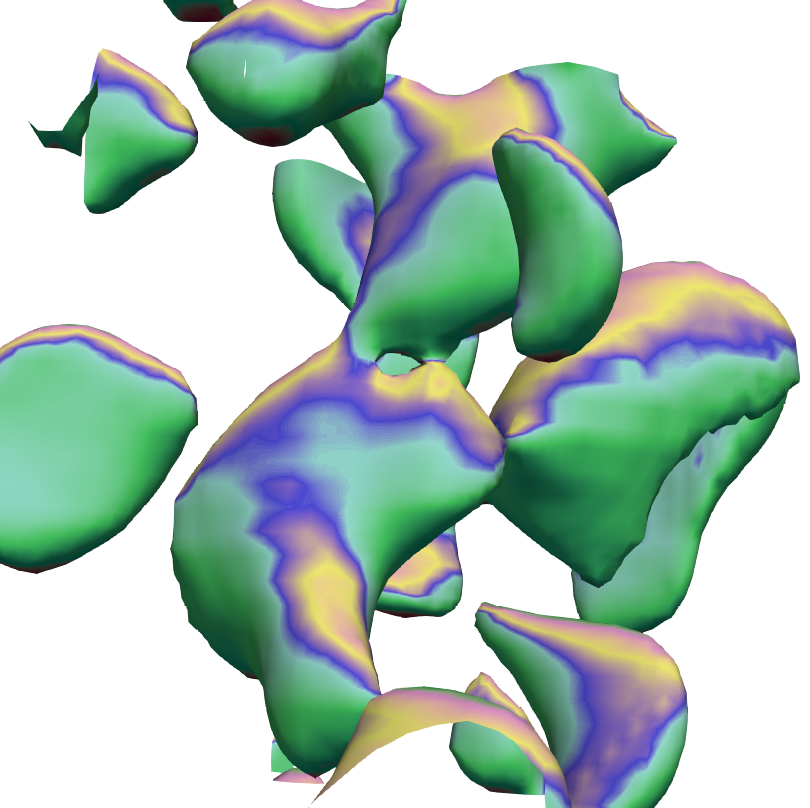
\includegraphics[width=0.16\linewidth]{isocontour/isocontour-bit-plane}}
\subcaptionbox{\emph{by wavelet norm} ($s_{wav}$)}
{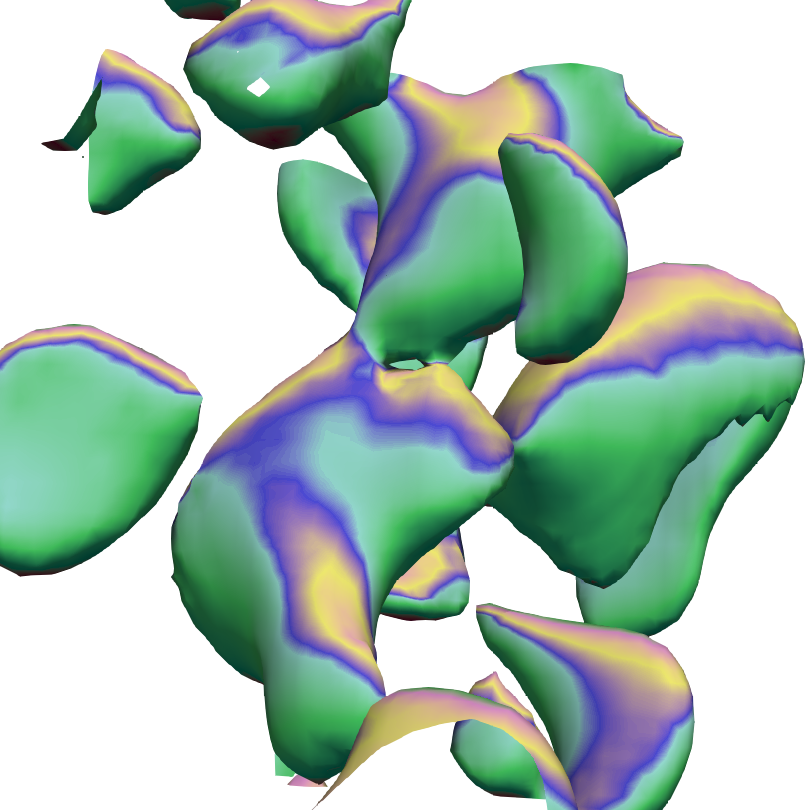
\includegraphics[width=0.16\linewidth]{isocontour/isocontour-wavelet-norm}}
\subcaptionbox{\emph{by magnitude} ($s_{mag}$)}
{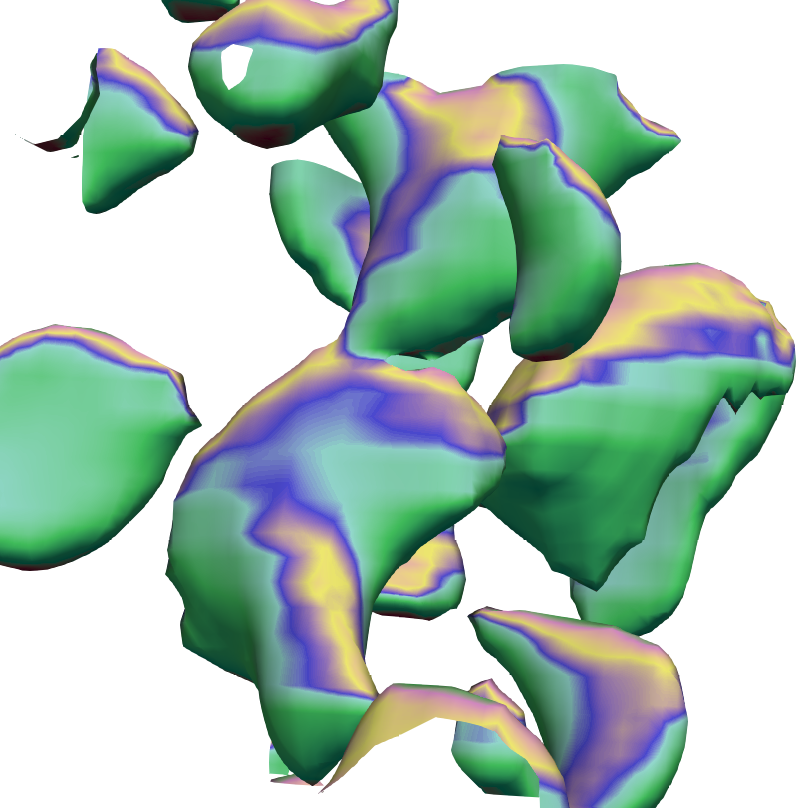
\includegraphics[width=0.16\linewidth]{isocontour/isocontour-magnitude}}
\subcaptionbox{\emph{by signature} ($s_{iso-sig}$)}
{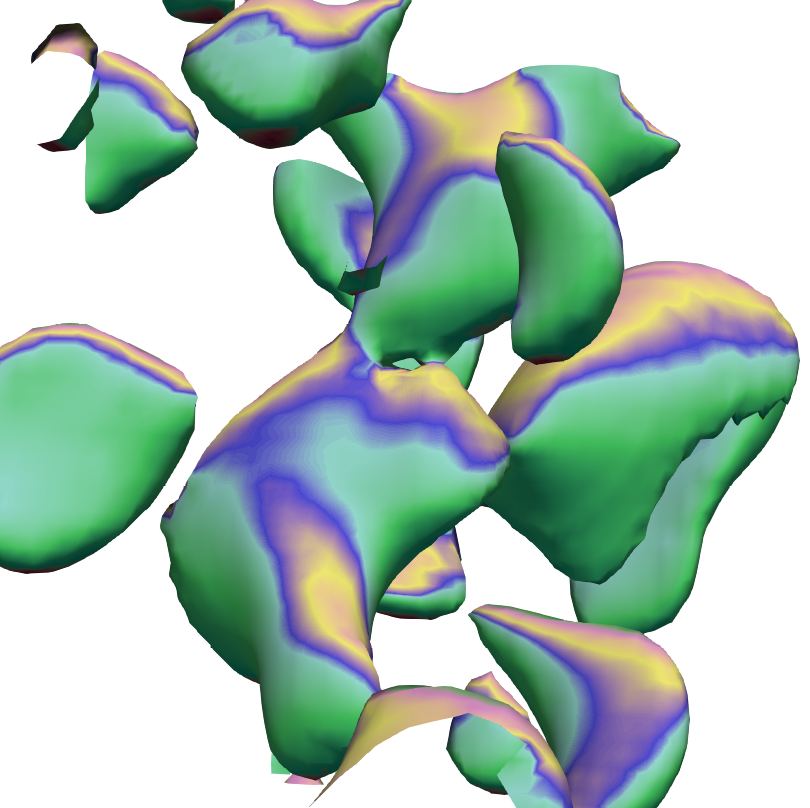
\includegraphics[width=0.16\linewidth]{isocontour/isocontour-signature}}
\subcaptionbox{\emph{ground truth}}
{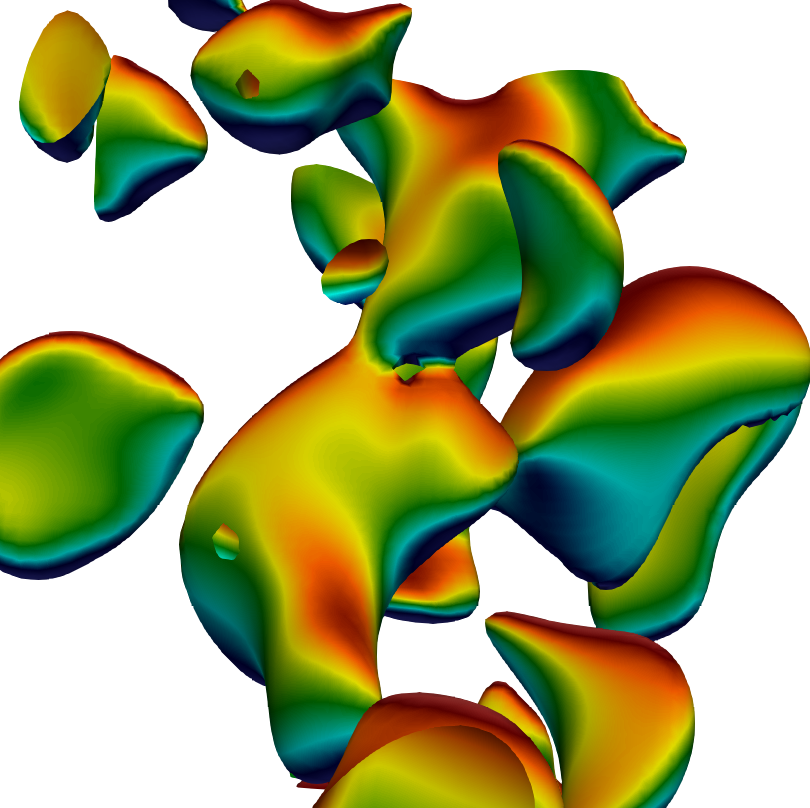
\includegraphics[width=0.16\linewidth]{isocontour/isocontour-groundtruth}} 
\caption{Rendering of isosurfaces at isovalue of 0.2, at 0.4 bps. The surfaces are colored by the
$x$-component of the normal vector at each point. The surfaces reconstructed by \swav and \sisg are
closest to the reference, followed by \sbit, \smag, and \slvl.}
\label{fig:isocontour-surfaces-pressure}
\end{figure*}

\begin{figure}[h]
\centering
\subcaptionbox{\emph{by bit plane} (\sbit)}
{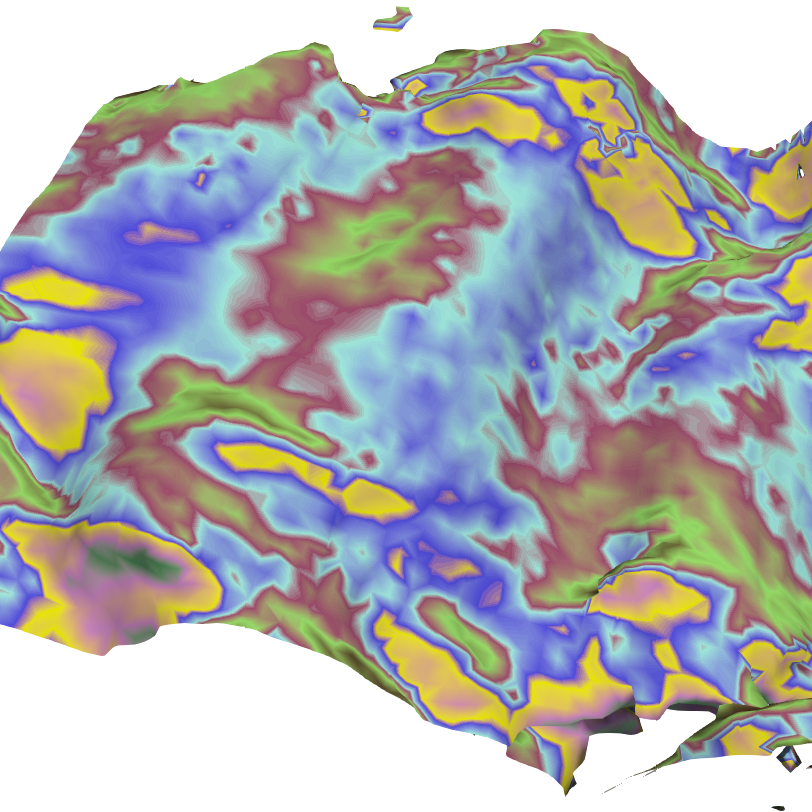
\includegraphics[width=0.32\linewidth]{isocontour/isocontour2-bit-plane}}
\subcaptionbox{\emph{by wavelet norm} (\swav)}
{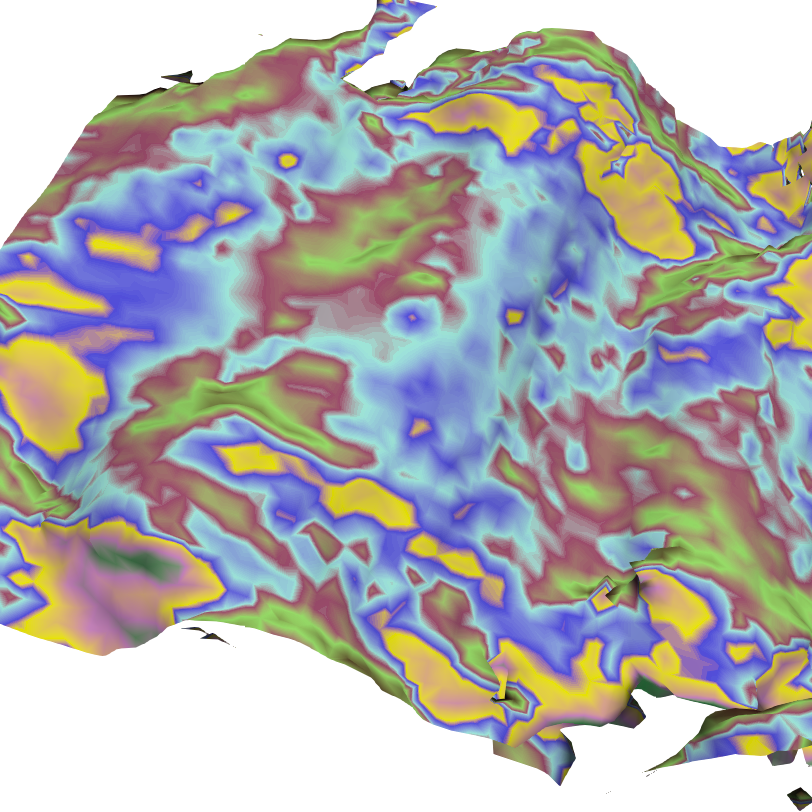
\includegraphics[width=0.32\linewidth]{isocontour/isocontour2-wavelet-norm}}
\subcaptionbox{\emph{ground truth}}
{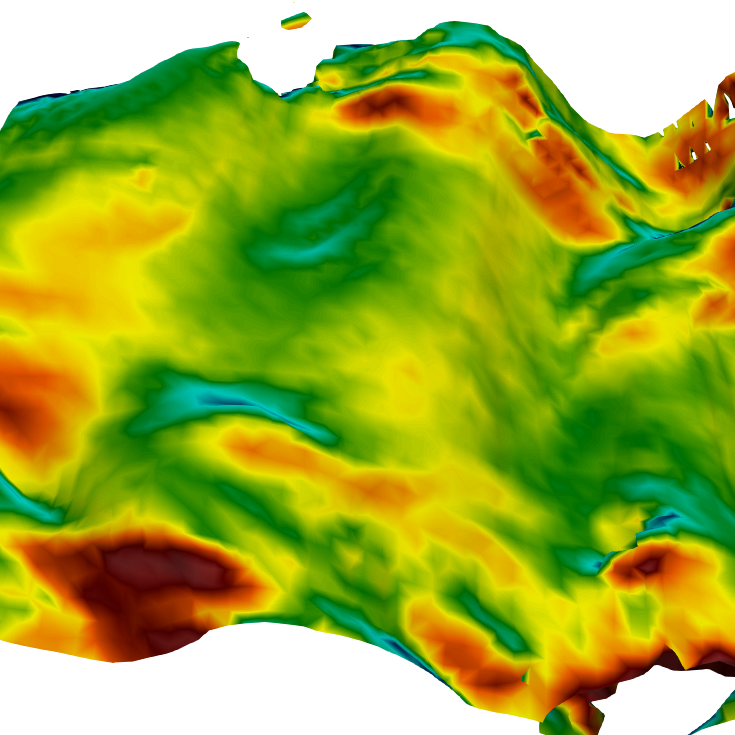
\includegraphics[width=0.32\linewidth]{isocontour/isocontour2-groundtruth}}
\caption{\emph{Plasma}'s isosurface reconstructed at 0.3 bps.}
\label{fig:isocontour-surfaces-plasma}
\end{figure}

Studying isosurfaces of a given function is an essential task in many visualization and analysis
pipelines, as they can highlight features of interest. For example, separation of burning and
extinguished regions can be performed by extracting isosurfaces of OH concentration.

Several sophisticated metrics exist that may be used to measure error in isosurface extraction,
focusing on different characteristics, including geometric~\cite{verifiable-isosurface} and
topological~\cite{topology-verification-isosurface} properties. Commonly used Hausdorff distance is
another choice, but is not very robust as it varies drastically with minor changes in the surfaces.
Since isosurfaces are also commonly used to partition the domain into ``inside'' and ``outside''
some region of interest, we opt for a simpler error metric that assumes nothing about the shape of
the isosurfaces, but simply counts misclassified voxels. However, since such a metric does not
capture the importance of a packet, the error caused by discarding that packet is of subvoxel
resolution. Therefore, in order to obtain an accurate error measurement to
support~\Cref{alg:greedy}, we add to the aforementioned error the relative difference in area,
$|A_1-A_2|/|A_1|$, between the two isosurfaces. The normalization reduces the range of this term to
$[0, 1]$, so that when the number of misclassified voxels is less than $1$, the subvoxel error is
instead captured by this relative difference in surface areas.

With the error metric defined, we compute a data-dependent stream optimized for that metric (\siop)
and a stream based on its signature (\sisg) using~\Cref{alg:greedy} and~\Cref{alg:signature}.
\Cref{fig:isocontour-plots} compares the performances of these two streams, along with \sbit, \slvl,
\swav, and \smag. As can be noticed, both \slvl and \smag perform poorly, indicating that
isosurface extraction favors resolution over precision. There are crossovers between \sbit and \swav
for the \emph{plasma} data set.

For this data set, the isosurface is extracted from a region with a low gradient, which means the
surface is very sensitive to low-ordered bits (i.e., a slight change in values moves the isosurface
by a larger distance). For this reason, \swav initially performs better, as it streams more precision
bits. As \sbit acquires enough precision, however, it starts to resolve the fine-scale geometry of
the surface better than \swav does (from~\autoref{fig:bit-plane-vs-wavelet-norm-gradient}
in~\Cref{sec:gradient}, we learn that \swav tends to reconstruct a smoother function everywhere).

\Cref{fig:isocontour-surfaces-plasma} shows the renderings of the surfaces reconstructed by \sbit
and \swav at 0.3 bps, which confirms that \sbit is able to preserve better the fine-scale featureas
on the surface. For the \emph{turbulence} field, the isosurface is extracted from a high-gradient
region; thus precision bits matter less, and \sbit outperforms \swav from the beginning. \sbit also
outperforms \sisg in this case, because local signatures coming from regions where the isosurface
does not intersect can dilute those coming from regions where it does. This phenomenon makes the
signature less useful for tasks that involve localization in the spatial domain, such as isosurface
extraction. Here, it happens in various degrees for every data set but it is especially relevant in
the case of \emph{turbulence}, since the surface is confined to very small regions of the whole
volume.

For a typical isosurface that is relatively smooth and is not too confined to small regions, such as
\emph{pressure} with an isovalue of 0.2, \swav typically outperforms \sbit
(see~\Cref{fig:isocontour-surfaces-pressure}). This figure renders the isosurfaces reconstructed at
0.4 bps for all streams. In terms of the quality of the reconstructed surfaces, $\sisg \approx \swav
> \sbit > \smag > \slvl$, which agrees with the curves in~\autoref{fig:isocontour-plots}. 
